\documentclass[12pt, a4paper]{scrartcl}

\usepackage{a4wide}
\usepackage{graphicx}      

\usepackage[utf8]{inputenc}
\usepackage[T1]{fontenc}
\usepackage[ngerman]{babel}

\renewcommand*\rmdefault{cmss}

\begin{document}
	
	\thispagestyle{empty}
	\null\vspace{40mm}
	\begin{center}
		{
			\Large  Die Nutzung von Vakuumpumpen für\\ unterschiedliche Anwendungen aufgrund ihrer Funktionsweise,\\ 
			sowie die Mechanik der Evakuierung	
			\footnote{
				\noindent Versuch F71, ausgeführt am 24.4.17,
				Betreuer: Frederik Arand,
				kurze besondere Auswertung
			}
		}\\[15mm]
		P. Nisblé und D. Bubeck
		
		\vspace{25mm}
		
		\parbox{0.9\textwidth}{
			Abstract:    
			\small The abstract should preferentially be in English. Here we explain in a
			few lines (i) what was done, and (ii) what the results were.
		}
	\end{center}
	
	\vfill
	Als besondere Auswertung testiert: Datum, Unterschrift:
	\vspace{20mm}
	
	%% Rueckseite des Titelblatts leer. Bei einseitigem Druck entfernen
	\newpage  
	\null\thispagestyle{empty} 
	
	%\newpage     % Inhaltsverzeichnis, koennte man bei langer Version machen
	%\tableofcontents 
	
	\newpage
	
	\pagenumbering{arabic} %% start page 1 
	\section{Einleitung}
		Diese Reihe von Versuchen dienen zur Orientierung und Nutzung von Apparaturen die Evakuierung benötigen, sowie zur Verständnis der Vakuumtechnik und auch deren Grenzen. In geringem Maße auch der Sensibilisierung für zuvor unbekannte Fehlerquellen die in der Vakuumtechnik zu Fehlern führen können.\\\\
		Der komplette Versuch ist getrennt in 6 Teilversuche:
		\begin{enumerate}
			\item Funktionsweise einer Drehschieberpumpe
			
				Beobachtung einer Drehschieberpumpe in Betrieb und Bbestimmung des maximalen Vakuums

			\item Abpumpen kondensierbarer Dämpfe
				
				Beobachtung der selben Drehschieberpumpe unter Abpumpen kondensierbarer Dämpfe und dem daraus resultierenden maximalen Vakuums

			\item Funktionsweise von Molekular- und Turbomolekularpumpe (TMP)
			
			\item Saugvermögen der TMP
			
			\item Bestimmung des Leitwerts von Rohr und Blende
			
			\item Lecksuche
		\end{enumerate}
	
	\section{Versuchsanordnung}
		\begin{figure}[h]
			\centering
			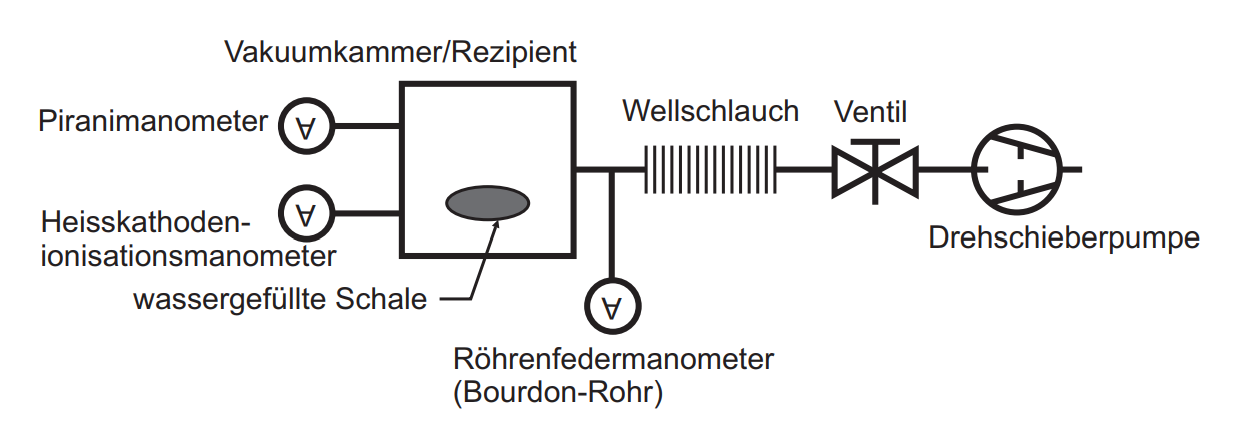
\includegraphics[width=.5\paperwidth]{aufbau22}
			\caption{Vakuum-Blockschaltbild zum Versuch des Abpumpens kondensierbarer Dämpfe}
		\end{figure}
	
		\begin{figure}[bh]
			\centering
			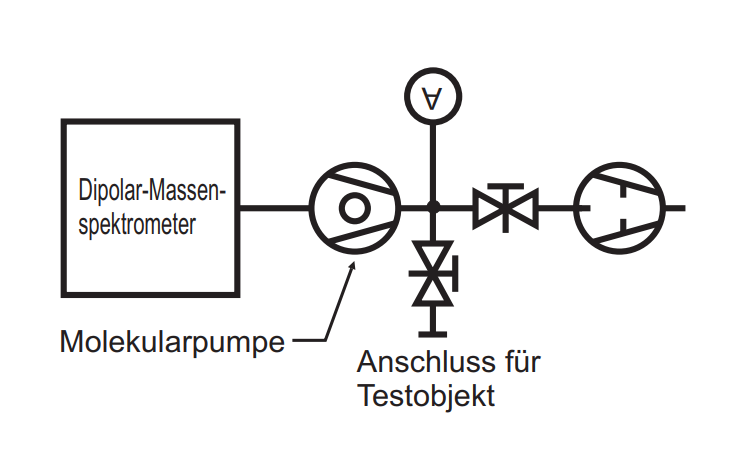
\includegraphics[width=.3\paperwidth]{aufbau262}
			\caption{Prinzipschaltbild des im Versuchsteil 6 eingesetzten Gegenstromlecksuchers}
		\end{figure}
		
	
	\section{Versuchsdurchführung}
	
	
	\subsection{Eichung}
	
	
	\section{Ergebnisse}
	
	
	
	\section{Diskussion}
	
	Hier werden alle wesentlichen Ergebnisse nochmals angefuehrt und diskutiert. 
	
	Am Schluss kann man noch eine allgemeinere Bemerkung zum Versuch machen.
	
	
	\newpage 
	
	\begin{thebibliography}{00}   % {00}: max 2-stellig
		
		\bibitem{afo} F. Afo, Nature 15 (1905) 23
		\bibitem{uwe} Uwe Ludwig, private Mitteilung
		\bibitem{karl} Karl Popper, Phys.~Rev.~Lett.~95 (2001) 25
		\bibitem{dipl} K. Winter, Diplomarbeit Heidelberg (1968)
		\bibitem{bibel} Genesis 3,4
		
	\end{thebibliography}
	
\end{document}